\documentclass[handout,t,compress]{beamer}
\usepackage{etex}
\usetheme{Singapore}

\sloppy
%\usepackage[scaled]{helvet}
%\usepackage{eulervm}

\usepackage{fp-eval}
\usepackage{hyperref}
\usepackage{fancyvrb}
\usepackage{pstricks,pst-node,pst-tree,pst-plot,pst-3dplot,multido}
\usepackage{graphicx}

\usepackage{alltt}


\newcommand{\bframe}[1]{\begin{frame}[fragile]{#1}}

\newcommand{\bbnf}{\begin{center}\begin{tabular}{rcl}}
\newcommand{\bnf}[2]{#1 & ::= & #2 \\}
\newcommand{\ebnf}{\end{tabular}\end{center}}

\newcommand{\myskip}{\vspace{-1em}\hrulefill}
\newcommand{\myrule}[1]{\vspace{-1ex}\centerline{\rule{#1cm}{1pt}}}
\newcommand{\myline}[1]{\centerline{#1}}
\newcommand{\bkt}[1]{\ensuremath{\langle\mbox{#1}\rangle}}
\newcommand{\br}{\mbox{~}|\mbox{~}}

\newcommand{\be}{\begin{eqnarray*}}
\newcommand{\ee}{\end{eqnarray*}}

\newcommand{\grph}[2]{
\begin{columns}
\column{0.01\textwidth}
\column{0.6\textwidth}
\begin{pspicture}[showgrid=#1](-2,-2)(5,5)
#2
\end{pspicture}
}

\newcommand{\txt}[1]{
\column{0.4\textwidth}
\rput[bl](0,0){\parbox{\textwidth}{
\footnotesize
\begin{itemize}
#1
\end{itemize}}}
\end{columns}}

\newcommand{\myvec}[1]{
\pstThreeDDot[showpoints=true,drawCoor=true](#1)
\pstThreeDLine[arrows=->,linecolor=blue](0,0,0)(#1)
}

\AtBeginSection[]
{
\bframe{Outline}
\tableofcontents[currentsection]
\end{frame}
}

\title{Game Physics Notes 01}
\author{CSCI 321}
\institute{WWU}

\begin{document}\small
\psset{arrowscale=2}

\bframe{~}
\titlepage
\end{frame}


\bframe{References}

{\footnotesize
  \begin{itemize}
  \item
    \url{http://tutorial.math.lamar.edu/Classes/CalcII/VectorsIntro.aspx}
  \item
    \url{http://chortle.ccsu.edu/vectorlessons/vectorindex.html}
  \item
    \url{https://www.mathsisfun.com/algebra/vectors.html}
  \item
    \url{https://unity3d.com/learn/tutorials/topics/scripting/vector-maths  }
  \end{itemize}
}
\end{frame}

\bframe{numpy}
A nice python library for dealing with mathematical vectors and matrices.

\begin{Verbatim}[frame=single]
>>> import numpy
>>> x = (1,2,3)
>>> y = (3,2,1)
>>> 3*x
(1, 2, 3, 1, 2, 3, 1, 2, 3)
>>> x + y
(1, 2, 3, 3, 2, 1)
>>> xvec = numpy.array(x)
>>> yvec = numpy.array(y)
>>> 3*xvec
array([3, 6, 9])
>>> xvec + yvec
array([4, 4, 4])
>>> numpy.dot(xvec, yvec)
10
\end{Verbatim}

\end{frame}

\bframe{Points in Space}

\grph{false}{
\psline[showpoints=true,linestyle=none](-1,1)(2,3)(1,0)(4,2)(1,4)
\rput[br](-1,1){$A$}
\rput[br](2,3){$B$}
\rput[br](1,0){$C$}
\rput[br](4,2){$D$}
\rput[br](1,4){$E$}
}

\txt{
\item Points exist in space without a coordinate system.
\item But with only labels it's difficult to compute with them.
}
\end{frame}

\bframe{Points in a Coordinate System}

\grph{true}{
\psline[showpoints=true,linestyle=none](-1,1)(2,3)(1,0)(4,2)(1,4)
\rput[br](-1,1){$A$}
\rput[br](2,3){$B$}
\rput[br](1,0){$C$}
\rput[br](4,2){$D$}
\rput[br](1,4){$E$}
}

\txt{
\item A coordinate system gives positions to points.
\item Relates {\em points} to {\em tuples of numbers}, or {\em
  mathematical vectors}.  
\item However, points are {\em not} vectors!
}
\end{frame}

\bframe{Different Coordinates}
\psset{unit=2cm}
\begin{columns}
\column{0.01\textwidth}
\column{0.6\textwidth}
\begin{pspicture}[showgrid=true](-1,-1)(2.5,2.5)
\psline[showpoints=true,linestyle=none](-0.5,0.5)(1,1.5)(0.5,0)(2,1)(0.5,2)
\rput[br](-.5,.5){$A$}
\rput[br](1,1.5){$B$}
\rput[br](.5,0){$C$}
\rput[br](2,1){$D$}
\rput[br](.5,2){$E$}
\end{pspicture}

\txt{
\item Different coordinate systems give different vectors,
 but the {\em points} are unchanged.
}
\psset{unit=1cm}
\end{frame}


\bframe{Physical vectors are differences between points.}

\grph{false}{
\psline[showpoints=true,linestyle=none](-1,1)(2,3)(1,0)(4,2)(1,4)
\rput[br](-1,1){$A$}
\rput[br](2,3){$B$}
\rput[br](1,0){$C$}
\rput[bl](4,2){$D$}
\rput[br](1,4){$E$}
\psline[arrows=->](-1,1)(2,3)
\rput[tl](.5,2){$\vec{v}=\overrightarrow{ab}=b-a$}
}
\txt{
\item Physical vectors are {\em not} mathematical vectors.
\item But given a coordinate system, you can represent the points as
  mathematical vectors, and then subtract.
\item But these mathematical vectors are not the same thing!
\item Different coordinate systems will give you different
  mathematical vectors for the {\em same} physical vector.
}
\end{frame}

\bframe{Points and vectors are not the same thing!}

\grph{false}{
\psline[showpoints=true,linestyle=none](-1,1)(2,3)(1,0)(4,2)(1,4)
\rput[br](-1,1){$A$}
\rput[br](2,3){$B$}
\rput[br](1,0){$C$}
\rput[bl](4,2){$D$}
\rput[br](1,4){$E$}
\psline[arrows=->](-1,1)(2,3)
\rput[tl](.5,2){$\vec{v}=\overrightarrow{ab}=b-a$}
}
\txt{
\item A point is a position in space.
\item A vector has a magnitude and a direction.
\item The vector from $a$ to $b$ is the point difference:
$\vec{v} = \overrightarrow{ab} = b-a$
\item  You can add two vectors, but  you {\em cannot} add two points!
\item You can add points and vectors: $b = a+\vec{v} = a + (b-a)$
}
\end{frame}

\bframe{Vector Addition}

\grph{false}{
\psline[showpoints=true,linestyle=none](-1,1)(2,3)(1,0)(4,2)(1,4)
\rput[br](-1,1){$A$}
\rput[br](2,3){$B$}
\rput[br](1,0){$C$}
\rput[bl](4,2){$D$}
\rput[br](1,4){$E$}
\psline[arrows=->](-1,1)(2,3)
\rput[br](.5,2){$B-A$}
\psline[arrows=->](2,3)(4,2)
\rput[bl](3,2.5){$D-B$}
\psline[arrows=->,linecolor=blue](-1,1)(4,2)
\rput[tl](1.5,1.5){$D-A = (B-A)+(D-B)$}
}
\txt{
\item vector + vector = vector
\item point + vector = point
\item point - point = vector
\item point + point = {\em nonsense}
}
\end{frame}

\bframe{Coordinates give mathematical vectors to physical vectors.}

\grph{true}{
\psline[showpoints=true,linestyle=none](-1,1)(2,3)(1,0)(4,2)(1,4)
\psline[arrows=<->](-1,1)(2,3)(4,2)
\psline[arrows=<->](1,0)(2,3)(1,4)
}
\txt{
\item Subtract the components.
\item $(1,4) - (2,3) = (-1, 1)$
\item $(-1,1) - (2,3) = (-1, -2)$
\item $(1,0) - (2,3) = (-1, -3)$
\item $(4,2) - (2,3) = (2,-1)$
\item Note: we subtract two {\em points} to get a
  {\em vector}. 
}
\end{frame}

\bframe{Vectors do not have positions}
\grph{true}{
\psline[arrows=->](-1,-1)(2,3)
\psline[arrows=->](1,-1)(4,3)
\psline[arrows=->](-1,1)(2,5)
\psline[arrows=->](0,0)(3,4)
}
\txt{
\item Each of these vectors is the {\em same} vector.
}

\end{frame}

\bframe{Vectors can be multiplied by scalars}
\grph{true}{
\psline[arrows=->](-1,2)(2,4)
\rput[ul](1,3){$\vec{v}$}
\psline[arrows=->](-1,0)(5,4)
\rput[ul](2.5,2){$2\vec{v}$}
\psline[arrows=->](4,1)(1,-1)
\rput[ul](3,0){$-\vec{v}$}
}
\txt{
\item Multiplication is repeated addition.
}
\end{frame}

\bframe{Lines}
\grph{false}{
\psline[linestyle=dotted](-2,-1)(5,2.5)
\psline[showpoints=true,linestyle=none](0,0)(4,2)
\psline[arrows=->,linecolor=blue](0,0)(2,1)
\rput[tl](0,0){$P$}
\rput[tl](1,.5){$\vec{v}$}
\rput[tl](4,2){$P + \alpha\vec{v}$}
}
\txt{
\item The line through $P$ in the direction $v$ is the set of all
  points $P+\alpha v$ for some $\alpha \in \mathbb{R}$
}
\end{frame}

\bframe{Planes (in 3 dimensions)}
\grph{false}{
\psline[linestyle=dotted](-2,-1)(5,2.5)
\psline[linestyle=dotted](0,-2)(0,5)
\psline[linestyle=dotted](3,1.5)(3,4)
\psline[linestyle=dotted](0,2.5)(3,4)
\psline[showpoints=true,linestyle=none](0,0)(3,4)
\psline[arrows=->,linecolor=blue](0,0)(2,1)
\psline[arrows=->,linecolor=blue](0,0)(0,2)
\rput[tl](0,0){$P$}
\rput[tl](1,.5){$\vec{v}$}
\rput[tr](0,1){$\vec{w}$}
\rput[bl](2,4){$P + \alpha\vec{v} + \beta\vec{w}$}
}
\txt{
\item The plane through $P$ spanned by $v$ and $w$ is the set of all
  points $P+\alpha v + \beta w$ for some $\alpha,\beta \in \mathbb{R}$
}
\end{frame}


\bframe{Affine sums}
\grph{false}{
\psline[linestyle=dotted](-2,-1)(5,2.5)
\psline[showpoints=true,linestyle=none](0,0)(2,1)(4,2)
\psline[arrows=->,linecolor=blue](0,0)(2,1)
\rput[tl](0,0){$P$}
\rput[tl](2,1){$Q$}
\rput[br](4,2){$\alpha_1 P + \alpha_2 Q$}
}
\txt{
\item
$P + \alpha(Q-P)$

$= (1-\alpha)P + \alpha Q$

$= \alpha_1 P + \alpha_2 Q$
\item $\alpha_1 + \alpha_2 = 1$
\item Think of each point as 
  the vector from some arbitrary point:

${P} \equiv P-O$

${Q} \equiv Q-O$

\item If $0 \leq \alpha_i$ then the point is between $P$ and $Q$.
}
\end{frame}
\bframe{Convex hull}
\grph{false}{


\pspolygon[showpoints=true,fillstyle=solid,fillcolor=lightgray](-1,-1)(2,0)(5,2)(4,4)(1,3)(-1,1)
\psline[showpoints=true,linestyle=none](1,1)(2,1)(3,3)(0,0)(3,2)
}
\txt{
\item $P= \alpha_1P_1 + \alpha_2P_2 + \ldots + \alpha_nP_n$
\item $\alpha_1 + \alpha_2 + \ldots + \alpha_n = 1$
\item $0 \leq \alpha_i$
}
\end{frame}

\bframe{Frames}

\grph{true}{
\psline[showpoints=true,linestyle=none](-1,1)(2,3)(1,0)(4,2)(1,4)
\psline[linecolor=blue,showpoints=true,arrows=->](0,0)(0,1)
\psline[linecolor=red,showpoints=true,arrows=->](0,0)(1,0)
}
\txt{
\item A coordinate system can be thought of as a single point, the
  {\em origin}, and a set of {\em basis vectors}.
\item Such a set is called a {\em frame}.
}
\end{frame}

\bframe{Frames}
\grph{true}{
\psline[showpoints=true,linestyle=none](-1,1)(2,3)(1,0)(4,2)(1,4)
\psline[linecolor=red,showpoints=true,arrows=->](0,0)(1,0)
\psline[arrows=->,linecolor=red](1,0)(2,0)
\psline[arrows=->,linecolor=blue](2,0)(2,1)
\psline[arrows=->,linecolor=blue](2,1)(2,2)
\psline[arrows=->,linecolor=blue](2,2)(2,3)
\rput[bl](2,3){$(2,3)$}
}
\txt{
\item The coordinates of a point are how many copies of the basis
  vectors you have to add to the origin.
}
\end{frame}

\bframe{Frames}
\grph{false}{
\psline[showpoints=true,linestyle=none](-1,1)(2,3)(1,0)(4,2)(1,4)
\psline[linecolor=red,showpoints=true,arrows=->](0,0)(1,0)
\psline[arrows=->,linecolor=red](1,0)(2,0)
\psline[arrows=->,linecolor=blue](2,0)(2,1)
\psline[arrows=->,linecolor=blue](2,1)(2,2)
\psline[arrows=->,linecolor=blue](2,2)(2,3)
\rput[bl](2,3){$(2,3)$}
}
\txt{
\item Note that a frame gives sense to coordinates without anything
  other than points and vectors.
\item A coordinate system is nothing more than an origin and a set of
  basis vectors, a {\em frame}.
\item An {\em orthonormal} frame is one in which all the vectors are
  of unit length and perpendicular to each other.
}
\end{frame}


\bframe{Frames do not have to be orthonormal}
\grph{false}{
\psline[linestyle=dotted](-2,-1)(5,2.5)
\psline[linestyle=dotted](0,-2)(0,5)
\psline[linestyle=dotted](3,1.5)(3,4)
\psline[linestyle=dotted](0,2.5)(3,4)
\psline[showpoints=true,linestyle=none](0,0)(3,4)
\psline[arrows=->,linecolor=blue](0,0)(2,1)
\psline[arrows=->,linecolor=blue](0,0)(0,2)
\rput[tl](0,0){$P$}
\rput[tl](1,.5){$\vec{v}$}
\rput[tr](0,1){$\vec{w}$}
\rput[bl](2,4){$Q = P + \alpha\vec{v} + \beta\vec{w} = (\alpha,\beta)$}
}
\txt{
\item The frame $F = (P,\vec{v},\vec{w})$ gives coordinates to any
  point in the plane it spans.  }
\end{frame}


\bframe{Trigonometry}
\grph{false}{
\psline(0,0)(4,0)(4,3)(0,0)
\psline[linecolor=.!25](3.5,0)(3.5,.5)(4,.5)
\psarc(0,0){1}{0}{36.67}
\rput[tl](2,-.1){$a$}
\rput[tl](4,1.5){$o$}
\rput(2,2){$h$}
\rput(1.2,.5){$\theta$}
}
\txt{
\item $\sin(\theta) = o/h$
\item $\cos(\theta) = a/h$
\item $\tan(\theta) = o/a$
}
\end{frame}

\bframe{Trigonometry}
\grph{false}{
\psline(0,0)(4,0)(4,3)(0,0)
\psline[linecolor=.!25](3.5,0)(3.5,.5)(4,.5)
\psarc(0,0){1}{0}{36.67}
\rput[tl](2,-.1){$h\cos(\theta)$}
\rput[tl](4,1.5){$h\sin(\theta)$}
\rput(2,2){$h$}
\rput(1.2,.5){$\theta$}
}
\txt{
\item $\tan(\theta) = \sin(\theta)/\cos(\theta)$
}
\end{frame}

\bframe{Trigonometry}
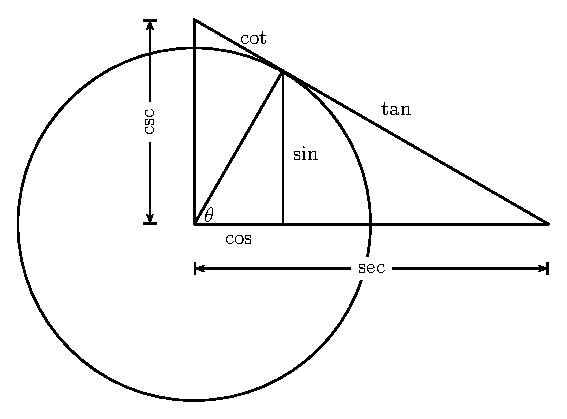
\includegraphics[scale=1]{Figures/trig.eps}
\end{frame}

\bframe{Dot product (Inner product)}
\grph{true}{
\psline[arrows=<->](5,0)(0,0)(3.2,3.2)
\psarc(0,0){1}{0}{45}
\rput[bl](1,.5){$\theta$}
\rput[bl](5,0){$\vec{u}$}
\rput[bl](3.2,3.2){$\vec{v}$}
}
\txt{
\item $u\cdot v = \cos(\theta)|u||v|$
\pause
\item $|u| = \sqrt{u\cdot u}$
}
\end{frame}

\bframe{Projection of one vector on another}
\grph{true}{
\psline[arrows=<->](5,0)(0,0)(3.2,3.2)
\psarc(0,0){1}{0}{45}
\rput[bl](1,.5){$\theta$}
\rput[bl](5,0){$\vec{u}$}
\rput[bl](3.2,3.2){$\vec{v}$}

\rput[t](3.2,-.1){$x$}
\psline[linestyle=dashed,linecolor=blue](3.2,0)(3.2,3.2)
}
\txt{
\item What is $x$?
}
\end{frame}

\bframe{Projection of one vector on another}
\grph{true}{
\psline[arrows=<->](5,0)(0,0)(3.2,3.2)
\psarc(0,0){1}{0}{45}
\rput[bl](1,.5){$\theta$}
\rput[bl](5,0){$\vec{u}$}
\rput[bl](3.2,3.2){$\vec{v}$}

\rput[t](3.2,-.1){$x$}
\psline[linestyle=dashed,linecolor=blue](3.2,0)(3.2,3.2)
}
\txt{
\item $x = \cos(\theta)|v|$
\item $x = {u\cdot v}/{|u|}$
}

\end{frame}

\bframe{Same direction, opposite direction}
\grph{false}{
\psline[arrows=<->](-2,2)(0,0)(5,0)
\psline[arrows=<->](0,3)(0,0)(4,2)
\psline[linestyle=dotted](0,-2)(0,5)
\rput[b](-2,2){$\vec{v_3}$}
\rput[b](0,3){$\vec{v_2}$}
\rput[b](4,2){$\vec{v_1}$}
\rput[l](5,0){$\vec{u}$}
}
\txt{
\item What is the sign of $u\cdot v_i$?
}

\end{frame}


\bframe{Same direction, opposite direction}
\grph{false}{
\psline[arrows=<->](-2,2)(0,0)(5,0)
\psline[arrows=<->](0,3)(0,0)(4,2)
\psline[linestyle=dotted](0,-2)(0,5)
\rput[b](-2,2){$\vec{v_3}$}
\rput[b](0,3){$\vec{v_2}$}
\rput[b](4,2){$\vec{v_1}$}
\rput[l](5,0){$\vec{u}$}
\rput[bl](4,3){Positive}
\rput[b](0,4){Zero}
\rput[bl](-2,3){Negative}
}
\txt{
\item Sign of $u\cdot v_i$ 
}
\end{frame}

\bframe{{\em AMAZING} theorem about the dot product.}
\begin{itemize}
\item In any coordinate system whatsoever:
\begin{eqnarray*}
u\cdot v &=& (u_x, u_y, u_z)\cdot (v_x, v_y, v_z) \\
&=& u_xv_x + u_yv_y + u_zv_z\\
&=& [u_x\  u_y\  u_z]\left[\begin{array}{c}v_x\\v_y\\v_z\end{array}\right]\\
&=& u^Tv
\end{eqnarray*}
\end{itemize}

\end{frame}

\bframe{Cross product (vector product)}
\grph{false}{
\psset{Alpha=60,showpoints=true,arrows=->,drawCoor=true}
\pstThreeDCoor
\myvec{0.5,2.0,-0.5}
\myvec{-1.0, 1.5, 0.5}
\myvec{1.75, 0.25, 2.75}
\pstThreeDPut(0.6,2.1,-0.7){$u$}
\pstThreeDPut(-1.1,1.6,0.6){$v$}
\pstThreeDPut(2,0,3){$u \times v$}
}
\txt{
\item A vector at right angles to $u$ and $v$.
\item $u \times v = $\\
$(u_2v_3 - u_3v_2,$\\$ u_3v_1 - u_1v_3,$\\$ u_1v_2 - u_2v_1)$

\item Mnemonic:
\[u\times v = \left|\begin{array}{ccc}
 \vec{i} & \vec{j} & \vec{k} \\
                           u_1 & u_2 & u_3 \\
                           v_1 & v_2 & v_3 \\
\end{array}\right|\]
\item $|u\times v| = |u||v|\sin(\theta)$
}
\end{frame}


\end{document}
